\documentclass{article}

\usepackage[utf8]{inputenc}

\usepackage{nicefrac}
\usepackage{amssymb, amsmath, amsfonts}
\usepackage{amsthm}
\usepackage{tikz}
\usetikzlibrary{matrix,shapes,arrows, calc, intersections}
\usetikzlibrary{decorations.markings}
\usepackage{pgfplots}
\usepgfplotslibrary{groupplots}
\usepackage[a4paper, margin=1in]{geometry}

\newtheorem{proposition}{Proposition}
\newtheorem{theorem}{Theorem}
\newtheorem{definition}{Definition}
\newtheorem{lemma}{Lemma}
\newtheorem{conjecture}{Conjecture}
\newtheorem{corollary}{Corollary}
\newtheorem{remark}{Remark}
\newtheorem{assumption}{Assumption}

\newlength\figureheight
\newlength\figurewidth
\setlength\figureheight{12cm}
\setlength\figurewidth{14cm}

\newcommand{\tikzdir}[1]{tikz/#1.tikz}
\newcommand{\inputtikz}[1]{\input{\tikzdir{#1}}}

\DeclareMathOperator*{\argmin}{arg\; min}     % argmin
\DeclareMathOperator*{\argmax}{arg\; max}     % argmax
\DeclareMathOperator*{\tr}{tr}     % trace
\DeclareMathOperator{\Cov}{Cov}
\DeclareMathOperator{\logdet}{log\;det}

\title{EE8087 Living with Mathematics\\Tutorial 4: Conic Sections}
\date{}
\begin{document} \maketitle
\begin{enumerate}
\item For a conic curve described by the following quadratic equation:
  \begin{align*}
    x^2 + 6xy+9y^2 + 2x - 5y + 10=0. 
  \end{align*}
  Calculate the eccentricity of the curve.

  \emph{Soln:} Notice that $\Delta_3 = -30.25\neq 0$ and $\Delta_2 = 0$. Therefore, the curve is a parabola and the eccentricity is $1$.

\item For a paper strip $AB$ of length $20$. Suppose $A$ is on the $y$-axis and $B$ is on the $x$-axis. If $P = (6,6)$ is on the paper strip, find the coordinate of $A$ and $B$.
\begin{figure}[ht]
  \centering
  \begin{tikzpicture}[scale=0.3]
 \draw[->] (0,0) -- (10,0) node[right] {$x$};
  \draw[->] (0,0) -- (0,20) node[above] {$y$};

  \node [inner sep=0, outer sep=0, label=90:$P$] (P) at (6,6) {}; 
  \fill [black] (P) circle (4pt); 

  \node [inner sep=0, outer sep=0, label=180:$A$] (a) at (0,17.84) {}; 
  \fill [black] (a) circle (4pt); 
  \node [inner sep=0, outer sep=0, label=270:$B$] (b) at (9.04,0) {}; 
  \fill [black] (b) circle (4pt); 

  \draw [semithick] (a)--(b);

  \node [inner sep=0, outer sep=0, label=180:$P'$] (PP) at (0,6) {}; 
  \fill [black] (PP) circle (4pt); 
  \draw [dashed] (P)--(PP);

  \node [inner sep=0, outer sep=0, label=180:$O$] (O) at (0,0) {}; 
  \fill [black] (O) circle (4pt); 
  \end{tikzpicture}
\end{figure}

\emph{Soln:} Let us assume that $AP = a$ and $PB = b$. Since $AB = 20$, $a+b = 20$. On the other hand, we know $P = (6,6)$ is on the following ellipse
\begin{align*}
  \frac{x^2}{a^2} + \frac{y^2}{b^2} = 1.
\end{align*}
Hence,
\begin{align*}
  1=\frac{36}{a^2}+\frac{36}{b^2}= 36\frac{a^2+b^2}{(ab)^2} = 36\frac{(a+b)^2-2ab}{(ab)^2} = 36\times\frac{400-2ab}{(ab)^2}.
\end{align*}
We can solve $ab = 89.28$. Therefore, $a$ and $b$ are the solutions of
\begin{align*}
  x^2 -20 x + 89.28 = 0.
\end{align*}
Solving the quadratic equation we get $a = 13.27$, $b = 6.73$ or $a = 6.73$, $b = 13.27$. Now since $\triangle AP'P$ and $\triangle AOB$ are similar, we have
\begin{align*}
  OB = \frac{PP'}{AP} AB = \frac{120}{a} = 9.04\text{ or }17.84.
\end{align*}
Similarly
\begin{align*}
  OA =  \frac{120}{b} = 17.84\text{ or }9.04.
\end{align*}

\item We have 3 base stations at $A = (-5,0)$, $B = (0,0)$ and $C = (5,0)$. Suppose the signal sends by the each station travels at a speed of $1$ and the three base stations broadcast the signal simultaneously at an unknown time. The signals from stations $A$, $B$ and $C$ are received by a boat at time $3$, $0$, $4$ respectively. Find the position of the boat $P$.

  \begin{figure}[ht]
    \centering
    \begin{tikzpicture}
      \draw[->] (6,0) -- (-6,0) node[right] {$x$};
      \draw[->] (0,-1) -- (0,4) node[above] {$y$};

      \node [inner sep=0, outer sep=0, label=45:$P$] (P) at (-0.529,1.706) {}; 
      \fill [black] (P) circle (2pt); 
      \node [inner sep=0, outer sep=0, label=270:$A$] (a) at (-5,0) {}; 
      \fill [black] (a) circle (2pt); 

      \node [inner sep=0, outer sep=0, label=45:$B$] (b) at (0,0) {}; 
      \fill [black] (b) circle (2pt); 

      \node [inner sep=0, outer sep=0, label=270:$C$] (c) at (5,0) {}; 
      \fill [black] (c) circle (2pt); 

      \draw (a)--(P)--(c);
      \draw (b)--(P);
    \end{tikzpicture}
  \end{figure}
  \emph{Soln} From the time of arrival data, we know that
  \begin{align*}
    PA-PB = 3.
  \end{align*}
  As a result, we know the locus of $P$ corresponds to the left branch of a hyperbola. The center of the hyperbola is $0.5A+0.5B = (-2.5,0)$ and $2c = 5$ and $2a = 3$. Therefore, $b = \sqrt{c^2-a^2}$ and the hyperbola is given by
  \begin{align}
    \label{eq:hyperbola1}
   \frac{(x+2.5)^2} {1.5^2}-\frac{y^2}{2^2} = 1.
  \end{align}
  Similarly, from $PC-PB = 4$, we know that $P$ is on the right branch of the following hyperbola
  \begin{align}
    \label{eq:hyperbola2}
   \frac{(x-2.5)^2} {2^2}-\frac{y^2}{1.5^2} = 1.
  \end{align}
  Cancelling the $y^2$ terms in \eqref{eq:hyperbola1} and \eqref{eq:hyperbola2} gives
  \begin{align*}
    4\frac{(x+2.5)^2} {2.25} - 2.25 \frac{(x-2.5)^2} {4} = 4-2.25,
  \end{align*}
  which is a quadratic equation of $x$. We can solve $x$ to be $-0.529$ or $-9.1$. Clearly $x=-9.1$ is incorrect since this will imply $P$ is closer to $A$ than to $B$ or $C$. For $x = -0.529$, we can solve $y = \pm 1.706$.


\newpage
\item We are building a Cassegrain reflector. Suppose the vertex of parabolic mirror is at $(0,0)$ and the vertex of the hyperbolic mirror is at $(5,0)$. The light is gathered at point $(-2,0)$. Find the equation describing the parabolic and hyperbolic mirrors.
  \begin{figure}[ht]
    \centering
    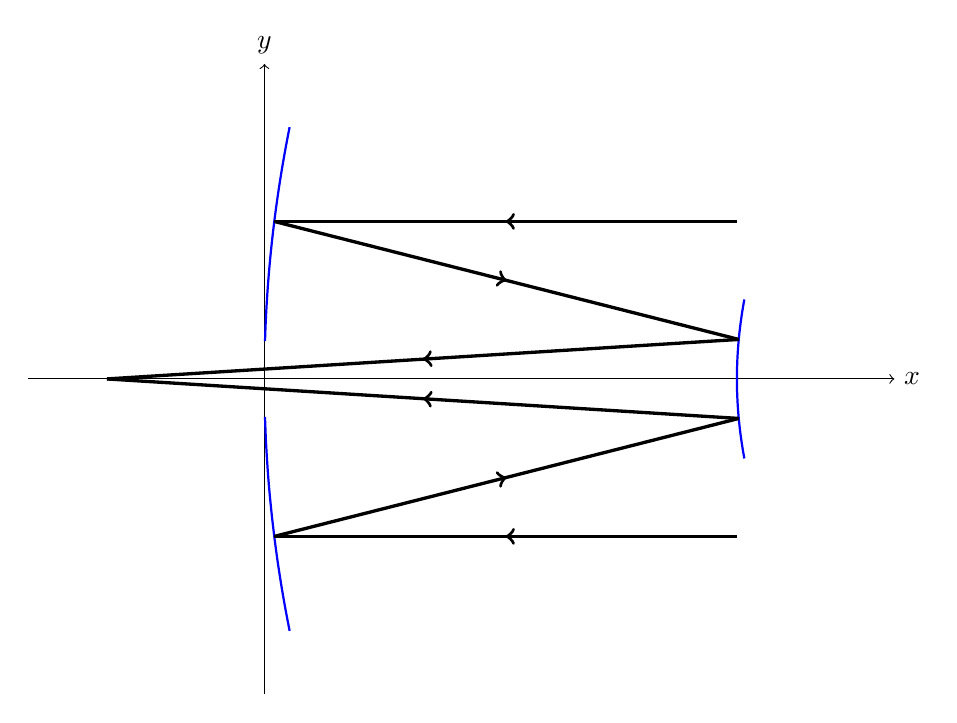
\begin{tikzpicture}
      \draw[->] (-3,0) -- (8,0) node[right] {$x$};
      \draw[->] (0,-4) -- (0,4) node[above] {$y$};

      \draw[name path=hyperbola, domain=-0.25:0.25, samples=20,smooth,variable=\t,blue,thick] plot ({3*cosh(\t)+3},{4*sinh(\t)});
      \draw[domain=-0.1:-0.015, samples=20,smooth,variable=\t,blue,thick] plot ({32*\t*\t},{32*\t});
      \draw[domain=0.015:0.1, samples=20,smooth,variable=\t,blue,thick] plot ({32*\t*\t},{32*\t});

      \path[name path=line1] (0.125,2)--(8,0);
      \path[name path=line2] (0.125,-2)--(8,0);
      \path[name intersections={of=line1 and hyperbola}];
      \begin{scope}[very thick,decoration={
          markings,
          mark=at position 0.5 with {\arrow{>}}}
        ] 
        \draw[postaction={decorate}] (6,2)--(0.125,2);
        \draw[postaction={decorate}] (0.125,2)--(intersection-1);
        \draw[postaction={decorate}] (intersection-1)--(-2,0);
      \end{scope}

      \path[name intersections={of=line2 and hyperbola}];
      \begin{scope}[very thick,decoration={
          markings,
          mark=at position 0.5 with {\arrow{>}}}
        ] 
        \draw[postaction={decorate}] (6,-2)--(0.125,-2);
        \draw[postaction={decorate}] (0.125,-2)--(intersection-1);
        \draw[postaction={decorate}] (intersection-1)--(-2,0);
      \end{scope}


    \end{tikzpicture}
  \end{figure}
  \emph{Soln:} Since the vertex of the parabola is $(0,0)$, the parabola is given by
  \begin{align*}
    y^2 = 4ax,
  \end{align*}
  with the focus at $(a,0)$.

  On the other hand, since the light being reflected by the hyperbola focuses at $(-2,0)$, we know that both $(a,0)$ and $(-2,0)$ are the foci of the hyperbola and the center of the hyperbola is at the middle point of the two foci: $(a/2-1,0)=(x_0,0)$. Assuming the hyperbola takes the following form
  \begin{align*}
    \frac{(x-x_0)^2}{A^2} - \frac{y^2}{B^2} = 1,\, C =\sqrt{A^2+B^2}.
  \end{align*}
  We know that
  \begin{align*}
    2C = a+2,\,C+A = 7.
  \end{align*}
  Therefore,
  \begin{align*}
    C = \frac{a}{2}+1,\,A = 6-\frac{a}{2}, B = \sqrt{C^2-A^2} = \sqrt{7(a-5)}.
  \end{align*}
  The equation for the hyperbola is
  \begin{align*}
    \frac{(x+1-a/2)^2}{(6-a/2)^2} - \frac{y^2}{7(a-5)} = 1.
  \end{align*}

  Notice that $a$ can be designed to be anything larger than $5$. Suppose $a = 8$, then the equations for the parabola and hyperbola are
\begin{align*}
  y^2 = 32x,\, \frac{(x-3)^2}{4} - \frac{y^2}{21} = 1.
\end{align*}

\end{enumerate}

\end{document}
%%% Local Variables:
%%% TeX-command-default: "Latexmk"
%%% End:
